\documentclass[11pt]{article}

% Change "review" to "final" to generate the final (sometimes called camera-ready) version.
% Change to "preprint" to generate a non-anonymous version with page numbers.
\usepackage[review]{acl}
\usepackage{amsmath}
\usepackage{enumitem}
\usepackage{pgfplots}
\pgfplotsset{compat=1.18}
% Standard package includes
\usepackage{times}
\usepackage{latexsym}
\usepackage{booktabs}
\usepackage{multirow}
\usepackage{makecell}
\usepackage{xcolor}
\usepackage{tcolorbox}
\usepackage{algorithm}
\usepackage{algpseudocode} % from algorithmicx
\usepackage{float}

% ruled style (top/bottom rules like the screenshot)
\floatstyle{ruled}
\restylefloat{algorithm}
\tcbuselibrary{skins,breakable}

\definecolor{mygreen}{RGB}{0,150,0}
\definecolor{myorange}{RGB}{230,120,0}
\definecolor{myred}{RGB}{200,0,0}

\newcommand{\step}[2]{\textbf{#1:}~#2\par}
\newcommand{\green}[1]{\textcolor{mygreen}{#1}}
\newcommand{\orange}[1]{\textcolor{myorange}{#1}}
\newcommand{\red}[1]{\textcolor{myred}{#1}}

\algnewcommand{\Input}{\item[\textbf{Input:}]}
\algnewcommand{\Output}{\item[\textbf{Output:}]}
\algnewcommand{\Parameters}{\item[\textbf{Parameters:}]}

% For proper rendering and hyphenation of words containing Latin characters (including in bib files)
\usepackage[T1]{fontenc}
% For Vietnamese characters
% \usepackage[T5]{fontenc}
% See https://www.latex-project.org/help/documentation/encguide.pdf for other character sets

% This assumes your files are encoded as UTF8
\usepackage[utf8]{inputenc}

% This is not strictly necessary, and may be commented out,
% but it will improve the layout of the manuscript,
% and will typically save some space.
\usepackage{microtype}

% This is also not strictly necessary, and may be commented out.
% However, it will improve the aesthetics of text in
% the typewriter font.
\usepackage{inconsolata}

%Including images in your LaTeX document requires adding
%additional package(s)
\usepackage{graphicx}

% If the title and author information does not fit in the area allocated, uncomment the following
%
%\setlength\titlebox{<dim>}
%
% and set <dim> to something 5cm or larger.

\title{D$^2$F-ReAG: Dynamic Decomposition and Filtering for Multi-Hop Reasoning-Augmented Generation}

% Author information can be set in various styles:
% For several authors from the same institution:
% \author{Author 1 \and ... \and Author n \\
%         Address line \\ ... \\ Address line}
% if the names do not fit well on one line use
%         Author 1 \\ {\bf Author 2} \\ ... \\ {\bf Author n} \\
% For authors from different institutions:
% \author{Author 1 \\ Address line \\  ... \\ Address line
%         \And  ... \And
%         Author n \\ Address line \\ ... \\ Address line}
% To start a separate ``row'' of authors use \AND, as in
% \author{Author 1 \\ Address line \\  ... \\ Address line
%         \AND
%         Author 2 \\ Address line \\ ... \\ Address line \And
%         Author 3 \\ Address line \\ ... \\ Address line}

\author{First Author \\
  Affiliation / Address line 1 \\
  Affiliation / Address line 2 \\
  Affiliation / Address line 3 \\
  \texttt{email@domain} \\\And
  Second Author \\
  Affiliation / Address line 1 \\
  Affiliation / Address line 2 \\
  Affiliation / Address line 3 \\
  \texttt{email@domain} \\}

%\author{
%  \textbf{First Author\textsuperscript{1}},
%  \textbf{Second Author\textsuperscript{1,2}},
%  \textbf{Third T. Author\textsuperscript{1}},
%  \textbf{Fourth Author\textsuperscript{1}},
%\\
%  \textbf{Fifth Author\textsuperscript{1,2}},
%  \textbf{Sixth Author\textsuperscript{1}},
%  \textbf{Seventh Author\textsuperscript{1}},
%  \textbf{Eighth Author \textsuperscript{1,2,3,4}},
%\\
%  \textbf{Ninth Author\textsuperscript{1}},
%  \textbf{Tenth Author\textsuperscript{1}},
%  \textbf{Eleventh E. Author\textsuperscript{1,2,3,4,5}},
%  \textbf{Twelfth Author\textsuperscript{1}},
%\\
%  \textbf{Thirteenth Author\textsuperscript{3}},
%  \textbf{Fourteenth F. Author\textsuperscript{2,4}},
%  \textbf{Fifteenth Author\textsuperscript{1}},
%  \textbf{Sixteenth Author\textsuperscript{1}},
%\\
%  \textbf{Seventeenth S. Author\textsuperscript{4,5}},
%  \textbf{Eighteenth Author\textsuperscript{3,4}},
%  \textbf{Nineteenth N. Author\textsuperscript{2,5}},
%  \textbf{Twentieth Author\textsuperscript{1}}
%\\
%\\
%  \textsuperscript{1}Affiliation 1,
%  \textsuperscript{2}Affiliation 2,
%  \textsuperscript{3}Affiliation 3,
%  \textsuperscript{4}Affiliation 4,
%  \textsuperscript{5}Affiliation 5
%\\
%  \small{
%    \textbf{Correspondence:} \href{mailto:email@domain}{email@domain}
%  }
%}

\begin{document}
\maketitle
\begin{abstract}
Large language models (LLMs) often generate inaccurate answers due to their static knowledge. Retrieval-augmented generation (RAG) addresses this by integrating external knowledge, excelling at single-hop queries. However, it struggles with multi-hop questions that require cross-document reasoning. Existing methods, such as graph-structured RAG or question decomposition, often lack dynamic decomposition and effective filtering, which leads to lower efficiency and accuracy. To overcome these limitations, we propose \textbf{D}ynamic \textbf{D}ecomposition and \textbf{F}iltering for Multi-Hop \textbf{Re}asoning-\textbf{A}ugmented \textbf{G}eneration (D$^2$F-ReAG), a novel paradigm that adaptively controls reasoning depth by judging the reliability of the root reasoning. If reliable, the question is solved. Otherwise, it is decomposed into sub-questions logically, and the correct reasoning for sub-questions updates the root reasoning. Experiments on three multi-hop benchmarks demonstrate the strong performance.
\end{abstract}

\section{Introduction}
Large Language Models (LLMs) have demonstrated strong understanding and generation abilities \cite{achiam2023gpt}, but they still struggle with knowledge updating and hallucinations \cite{jiang-etal-2024-large}. Retrieval-augmented Generation (RAG) mitigates this by injecting external knowledge into generation \cite{lewis2020retrieval}.

For simple questions, retrievers often find relevant evidence in one step \cite{shi-etal-2024-generate}. In contrast, multi-hop reasoning requires separated facts \cite{cheng-etal-2025-dualrag}. Graph-based RAG (Graph RAG) connects facts via pre-built graphs \cite{edge2024local}, but these graphs may be incomplete and difficult to maintain \cite{li2025subqrag}.

Recent advances such as LogicRAG \cite{chen2025you} reduce the reliance on pre-constructed graphs by decomposing complex queries into sub-questions and iteratively compressing retrieved evidence into a document-level memory. Nevertheless, such compression does not fully filter out redundant or erroneous information in the resulting memory \cite{zhuang-etal-2024-efficientrag}, and the query decomposition process is often inflexible, leading to degraded reasoning performance \cite{kim-etal-2025-unirag}.

\begin{figure*}[t]
  \centering
  
\includegraphics[width=\textwidth]{ReAG.pdf}
    \caption{The D$^2$F-ReAG framework consists of four stages: (I) Retrieval \& Generation, which retrieves relevant documents to generate a reasoning. (II) Judge Reliability, where an LLM evaluates reasoning reliability against a threshold. (III) Decomposition \& Rewriting, which decomposes and rewrites the question when reliability is insufficient. (IV) ReAG (Reasoning augments generation), which integrates reliable and relevant sub-question reasoning to update the root reasoning. The process stops once the root question is answered reliably.}
  \label{fig:pdf_image}
\end{figure*}
We propose D$^2$F-ReAG, a multi-hop reasoning framework that dynamically performs on-demand question decomposition and augments generation with reliable sub-question reasoning. Specifically, D$^2$F-ReAG decomposes a question only when its reasoning is unreliable. Once a sub-question is solved reliably and considered relevant, it is used to update and guide the reasoning of the root question. D$^2$F-ReAG stops early once the root question is answered reliably to avoid over-reasoning. In summary, our contributions are:
\begin{itemize}
    \item We propose D$^2$F-ReAG, a framework that dynamically decomposes sub-questions and augments the root question's reasoning with correct reasoning processes of sub-questions.
    \item We dynamically balance the decomposition depth between simple and complex questions, enabling on-demand decomposition.
\item We use reliable sub-questions' reasoning to update the root reasoning to reduce error.
\end{itemize}

\section{Related Work}
Graph RAG includes GraphRAG \cite{edge2024local}, which uses hierarchical community search with local and global queries, and LightRAG \cite{guo-etal-2025-lightrag}, which improves large-scale retrieval via a two-stage, graph-augmented index. RAPTOR \cite{sarthi2024raptor} builds hierarchical summaries for multi-granular retrieval. HippoRAG \cite{gutiérrez2024hipporag} and HippoRAG 2 \cite{gutiérrez2025ragmemorynonparametriccontinual} improve long-context coherence using PageRank \cite{page1999pagerank} node ranking and paragraph-level memory integration.

Prompt-based RAG methods \cite{chang2024efficient} interleave reasoning and retrieval via prompting. 
ReAct \cite{yao2023react} alternates reasoning with retrieval. ChainRAG \cite{zhu-etal-2025-mitigating} uses prompt-guided sub-question decomposition and iterative sentence-graph retrieval; and LogicRAG \cite{chen2025you} decomposes questions and aggregates multi-step evidence. SiGIR \cite{chu-etal-2025-self} refines reasoning iteratively, but decomposes by atomicity and lacks explicit correctness checks.

\section{Method}

We propose D$^2$F-ReAG, a dynamic framework for multi-hop reasoning. As shown in Figure~\ref{fig:pdf_image} and Appendix \ref{sec:Pseudo Code}, D$^2$F-ReAG begins with (I) Retrieval \& Generation, where first retrieves top-$k$ documents to generate question's reasoning. In (II) Judge Reliability, a judge model evaluates the reliability of the reasoning. If reliable, the question is solved; otherwise, (III) Decomposition \& Rewriting decomposes the question into sub-questions and rewrites them to retrieve more relevant evidence. Finally, (IV) ReAG (Reasoning-Augmented Generation) augments root reasoning with reliable, relevant reasoning traces of sub-questions. D$^2$F-ReAG stops once the root reasoning score exceeds a threshold.

\subsection{Retrieval \& Generation}

For the root question $q_{root}$ and each sub-question $q_i$, we retrieve the top-$k$ documents $D(q)$ from the corpus $\mathcal{C}$ and generate the corresponding reasoning process $r(q)$. Formally, for any question $q \in \{q_{root}, q_1, \dots, q_n\}$,
\begin{equation}
r(q) = \mathrm{Generator}\bigl(q, D(q)\bigr),
\end{equation}
where $\mathrm{Generator}$ denotes the model that generates detailed reasoning based on relevant documents.
\subsection{Judge Reliability}
After generating the reasoning for the root or sub-questions, we judge its reliability using an LLM-based scoring mechanism. We denote the reliability score of the reasoning process as \( s_r(q) \), which is calculated by LLM:
\begin{equation}
    s_r(q) = \text{Score}(q, r(q)),
\end{equation}
where \( r(q) \) represents the reasoning process, and \( \text{Score}(q, r(q)) \) is the reasoning score provided by the LLM according to the rubric in Appendix \ref{sec:prompt}.

The reasoning score $s_r(q) \in [0,10]$ measures reasoning reliability (higher is better). We compare it to a threshold $\theta$: if $s_r(q) > \theta$, we consider the question solved. Otherwise, D$^2$F-ReAG thinks the reasoning unreliable and further decomposes the question for continued reasoning (Section~\ref{sec:decomposition})
\begin{equation}
    \mathrm{Judge} =
    \begin{cases}
    \text{Solved}, & \text{if } s_r(q) > \theta \\
    \text{Decompose}, & \text{if } s_r(q) \leq \theta.
    \end{cases}
\end{equation}

% By judging reliability, unresolved questions are decomposed for further reasoning (Section~\ref{sec:decomposition}), while reliably solved and relevant sub-questions update the root reasoning in ReAG (Section~\ref{sec:reag}).
If the current question is the root question and is deemed solved, the LLM generates the final answer based on the corresponding reasoning process
\begin{equation}
a_{\text{root}} = \text{Answer}\!\left(r_{q_{\text{root}}}\right).
\label{eq:root_answer}
\end{equation}

If a sub-question is reliably solved, we use its relevant sub-questions to update the root reasoning in ReAG (Section~\ref{sec:reag}).

\subsection{Decomposition \& Rewriting}
\label{sec:decomposition}
When the root question or any sub-question remains unsolved, we use prompt engineering to logically decompose it into smaller sub-questions.
\begin{equation}
sub(q) = \text{Decompose}(q),
\end{equation}
where $sub(q)$ is the set of sub-questions obtained by decomposing the question $q$.

D$^2$F-ReAG first solves each sub-question in order and judges the reliability of the reasoning. If reliable, we rewrite the related other sub-questions $q \in \mathcal{S}_i$ based on the correct reasoning $r_q$. 
\begin{equation}
\mathcal{S}_i' = \{\, \text{Rewrite}(q, r_q) \mid q \in \mathcal{S}_i \,\},
\label{eq:rewrite}
\end{equation}
where $r_q$ is the reasoning to the current question, and $q_i$ is the related sub-question.

\subsection{ReAG}
\label{sec:reag}
When a sub-question is solved reliably, we check its relevance to the root question and use its reasoning to update the root reasoning if relevant.
\begin{equation}
\text{Check}(q_i, q) = 
    \begin{cases}
    \text{relevant} \\
    \text{irrelevant} 
    \end{cases}
\end{equation}
where Check$(q_i, q)$ represents the relevance between the sub-question $q_i$ and the root $q$.

If a sub-question’s reasoning is reliable and relevant, it is used to update the root reasoning. Formally, this can be written as:
\begin{equation}
r(q_{root}' = \text{Update}(r(q_{root}), r(q)),
\label{eq:update}
\end{equation}
where \( r(q_{root})' \) is the updated reasoning process of the root problem \( q \), \( r(q) \) is the reasoning process of the sub-question \( q_i \), and \( \text{Update}(r(q_{root}), r(q)) \) updates \( r(q_{root}) \) by incorporating \( r(q) \). 

Once the root reasoning is reliable, we stop processing the remaining sub-questions and obtain final answer to avoid over-reasoning.

\begin{table*}
  \centering
  \renewcommand{\arraystretch}{0.85}
  \setlength{\tabcolsep}{3.5pt}
  \begin{tabular}{l l c c c c c c}
    \toprule
    \multirow{2}{*}{\textbf{Baseline Type}} & \multirow{2}{*}{\textbf{Method}} &
    \multicolumn{2}{c}{\textbf{HotpotQA}} &
    \multicolumn{2}{c}{\textbf{2Wiki}} &
    \multicolumn{2}{c}{\textbf{MuSiQue}} \\
    \cmidrule(lr){3-4} \cmidrule(lr){5-6} \cmidrule(lr){7-8}
    & & \textbf{Str-Acc} & \textbf{LLM-Acc} & \textbf{Str-Acc} & \textbf{LLM-Acc} & \textbf{Str-Acc} & \textbf{LLM-Acc} \\
    \midrule

    \multirow{4}{*}{Zero-shot} & Llama3 (8b) & 17.1 & 11.1 & 22.3 & 4.7 & 2.3 & 2.0 \\
    & Llama3 (13b) & 23.7 & 20.1 & 33.8 & 15.4 & 6.4 & 6.0 \\
    & gpt-3.5-turbo & 31.5 & 35.4 & 24.0 & 22.0 & 7.9 & 10.9 \\
    & gpt-4o-mini & 38.7 & 36.3 & 26.4 & 24.3 & 17.6 & 14.0 \\

    \midrule
    \multirow{5}{*}{Graph-based} & RAPTOR & 48.1 & 57.8 & 47.7 & 45.9 & 25.2 & 29.1 \\
    & GraphRAG & 39.6 & 45.2 & 46.3 & 43.3 & 16.5 & 19.4 \\
    & LightRAG & 47.8 & 57.7 & 43.1 & 36.3 & 18.1 & 19.4 \\
    & HippoRAG & 53.5 & 56.6 & 47.2 & 47.2 & 24.9 & 30.1 \\
    & HippoRAG2 & \textbf{56.7} & 61.9 & 50.0 & 47.1 & 27.0 & 32.6 \\

    \midrule
    \multirow{4}{*}{Prompt-based RAG} & VanillaRAG & 43.2 & 53.1 & 43.0 & 42.0 & 20.3 & 23.6 \\
    & ReAct$^\dagger$ & 54.2 & 56.5 & 54.9 & 50.8 & 28.8 & 31.9 \\
    & ChainRAG$^\dagger$ & 52.1 & 56.6 & \underline{68.9} & \underline{66.2} & \underline{31.0} & 33.8 \\
    & LogicRAG$^\dagger$ & 54.2 & \underline{62.5} & 65.3 & 62.6 & 29.6 & \underline{36.5} \\

    \midrule
    Our proposed & D$^2$F-ReAG & \underline{55.8} & \textbf{63.4} & \textbf{70.3} & \textbf{68.9} & \textbf{32.2} & \textbf{37.9} \\
    \bottomrule
  \end{tabular}
  \caption{Performance comparison of different methods on HotpotQA, 2WikiMultiHopQA and MuSiQue using Str-Acc and LLM-Acc. The results of the methods marked with † are from our own reimplementation, others are from the LogicRAG implementation. The best and second-best results are marked in bold and underlined.}
  \label{tab:accents}
\end{table*}


\section{Experiments}
\subsection{Experiment Setup}
\textbf{Dataset.}
We evaluate on three standard multi-hop reasoning benchmarks: HotpotQA \cite{yang-etal-2018-hotpotqa}, MuSiQue \cite{trivedi2021musique} and 2WikiMultiHopQA \cite{ho-etal-2020-constructing}, covering diverse cross-document and multi-hop reasoning. Following HippoRAG~2 \cite{gutiérrez2025ragmemorynonparametriccontinual}, we use the same retrieval corpus and randomly sample 1,000 questions from each validation set for evaluation, ensuring fair comparison.

\textbf{Baseline.}
We compare D$^2$F-ReAG with three categories of baselines: \textbf{Zero-shot} (llama3(8B), llama3(13B) \cite{dubey2024llama}, gpt-3.5-turbo, gpt-4o-mini \cite{achiam2023gpt}). \textbf{Graph RAG} (KGP \cite{wang2024knowledge}, G-retriever \cite{he2024g}, RAPTOR \cite{sarthi2024raptor}, GraphRAG \cite{edge2024local}, LightRAG \cite{guo-etal-2025-lightrag}, HippoRAG \cite{gutiérrez2024hipporag} and HippoRAG 2 \cite{gutiérrez2025ragmemorynonparametriccontinual}). \textbf{Prompt-based} RAG (ReAct \cite{yao2023react}, ChainRAG \cite{zhu-etal-2025-mitigating}, and LogicRAG \cite{chen2025you}).

\textbf{Metrics.} Following LogicRAG, we report Str-Acc (normalized exact match) and LLM-Acc (LLM-based semantic correctness).


\textbf{Implementation Details.} All methods use the same embedding model (sentence-transformers/all-MiniLM-L6-v2) \cite{wang-etal-2021-minilmv2} with top-$k$ set to 3 and use gpt-4o-mini \cite{achiam2023gpt} for generation on a single NVIDIA RTX 3090 GPU.



\subsection{Main Results}
Table~\ref{tab:accents} reports results on three multi-hop reasoning benchmarks. D$^2$F-ReAG achieves the best or near-best performance on Str-Acc and LLM-Acc.

Zero-shot LLMs improve with stronger backbones but still trail retrieval-based methods, underscoring the need for external evidence. Graph-based RAG (GraphRAG, RAPTOR, LightRAG, HippoRAG and HippoRAG 2) boosts performance by structuring context. ChainRAG combines sub-question decomposition with sentence-graph retrieval, leading to stronger multi-hop QA performance. Prompt-based RAG like ReAct and LogicRAG further improves multi-hop reasoning by interleaving retrieval and reasoning. However, these methods remain limited by fixed decomposition depth and retrieval noise.

D$^2$F-ReAG achieves the best performance on 2Wiki and MuSiQue and the highest LLM-Acc on HotpotQA, with the largest gains on 2WikiMultiHopQA, demonstrating the effectiveness of on-demand decomposition and reliability-guided reasoning. We report the best scores across runs, with a detailed case study in Appendix \ref{sec:appendix}.
\begin{figure}[t]
\centering
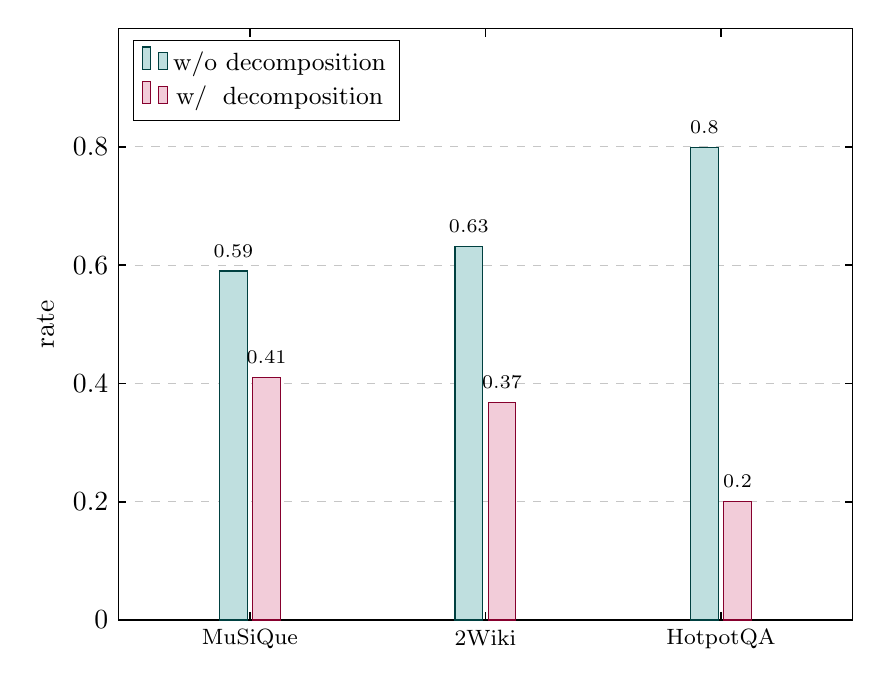
\begin{tikzpicture}
\begin{axis}[
    ybar,
    bar shift auto,
    width=0.9\columnwidth,
    height=0.75\columnwidth,
    ymin=0, ymax=1,
    ytick={0,0.2,0.4,0.6,0.8},
    ylabel={rate},
    ymajorgrids,
    grid style={dashed,gray!45},
    xticklabel style={font=\footnotesize},
    axis lines=box,          
    tick align=inside,     
    tick style={black, line width=0.6pt},
    major tick length=3pt,
    symbolic x coords={MuSiQue,{2Wiki},HotpotQA},
    xtick=data,
    enlarge x limits=0.28,
    bar width=10pt,
    legend style={
        at={(0.02,0.98)},
        anchor=north west,
        legend columns=1,
        draw=black,
        fill=white,
        font=\small,
        inner xsep=3pt,
        inner ysep=2pt
    },
    nodes near coords={\pgfmathprintnumber[fixed,precision=2]{\pgfplotspointmeta}},
    point meta=y,
    every node near coord/.append style={font=\scriptsize, yshift=1.5pt,text=black},
]

\addplot+[fill=teal!25, draw=teal!50!black] coordinates {
    (MuSiQue,0.59)
    ({2Wiki},0.632)
    (HotpotQA,0.799)
};
\addlegendentry{w/o decomposition}

\addplot+[fill=purple!20, draw=purple!70!black] coordinates {
    (MuSiQue,0.41)
    ({2Wiki},0.368)
    (HotpotQA,0.201)
};
\addlegendentry{w/\; decomposition}

\end{axis}
\end{tikzpicture}
\caption{Proportion of questions solved with decomposition and without decomposition on three benchmarks.}
\label{fig:pdf_image_rate}
\end{figure}

\begin{table}[htbp]
\centering
\renewcommand{\arraystretch}{0.9}
\setlength{\tabcolsep}{3.5pt}
\begin{tabular}{l c c c c}
\toprule
\textbf{Method}
& \makecell{\textbf{Str}\\\textbf{Acc}}
& \makecell{\textbf{LLM}\\\textbf{Acc}}
& \makecell{\textbf{Avg.}\\\textbf{Time (s)}}
& \makecell{\textbf{Avg.}\\\textbf{Tokens}} \\
\midrule
ReAct        & 54.9 & 50.8 & 13.93 & 11287 \\
LogicRAG     & 65.3 & 62.6 & 15.35 & 1998  \\
\midrule
Ours (No D)  & 71.9 & 71.0 & 9.49  & 2267  \\
Ours (+D)    & 67.3 & 65.0 & 73.54 & 13321 \\
Ours (Avg.)  & 70.3 & 68.9 & 32.4  & 6057  \\
\bottomrule
\end{tabular}
\caption{Accuracy and efficiency comparison on 2WikiMultiHopQA (with vs. without decomposition).}
\label{tab:2wiki_efficiency}
\end{table}
\subsection{Decomposition \& Efficiency Comparison}
Figure \ref{fig:pdf_image_rate} shows that a large proportion of questions can be solved without decomposition, demonstrating the necessity of dynamic decomposition to efficiently handle both simple and complex questions.\\
Since ChainRAG also uses a pre-built sentence graph, we compare latency and efficiency with ReAct and LogicRAG. Table \ref{tab:2wiki_efficiency} shows that always decomposing and judging reliability greatly increases time and token cost. In contrast, on-demand decomposition skips unnecessary steps, speeding up easy cases while still decomposing for hard ones. While our multi-step judgments can take longer on some difficult examples, Figure \ref{fig:pdf_image_rate} confirms these long cases are relatively few. Overall, D$^2$F-ReAG balances between performance and efficiency and better matches human-like reasoning.


\section{Conclusion}
Existing RAG exhibit limitations in using fixed decomposition and filtering out error or irrelevant information. Therefore, we propose D$^2$F-ReAG (Dynamic Decomposition and Filtering for Multi-Hop Reasoning-Augmented Generation), a framework that dynamically decomposes questions only when necessary and filters reasoning based on reliability. By integrating correct reasoning of sub-questions to augment root generation, D$^2$F-ReAG demonstrates strong performance for multi-hop questions.  
\section{Limitations}
Reasoning reliability judging causes additional token cost, which could be reduced by using smaller or open-source models for simple steps. Some errors also result from weak retrieval or ineffective use of retrieved evidence, indicating the need for stronger retrievers and generators in future work.

LLM-based scoring may sometimes judge a reasoning trace incorrectly. We believe these errors mainly come from the LLM’s limited ability and randomness in its outputs, and more reliable verification or better-designed scoring models could further improve robustness.

% Bibliography entries for the entire Anthology, followed by custom entries
%\bibliography{anthology,custom}
% Custom bibliography entries only
\bibliography{custom}

\appendix

\onecolumn
\section{Case Study}
\label{sec:appendix}
In this section, we present a case study to compare the reasoning behaviors of \textbf{D$^2$F-ReAG} and \textbf{LogicRAG}.

\begin{figure*}[h!]
\centering
\begin{minipage}{0.98\textwidth}
\begin{tcolorbox}[
  breakable,
  colback=white,
  colframe=black,
  boxrule=0.8pt,
  arc=1pt,
  left=6pt,right=6pt,top=6pt,bottom=6pt
]

\textbf{Question: }{Which film has the director who died later, {45 Calibre Echo} or {Bons Baisers De Hong Kong}?}\\
\textbf{Gold Answer: }{{Bons Baisers De Hong Kong}}\\
Failure Case of \textbf{LogicRAG}.\\
\textbf{Model Answer: }{\textcolor{red}{\textit{45 Calibre Echo}} \;(\textbf{Incorrect})}\\
{Rounds}{ 1}

\step{Retrieved Contexts}{
LogicRAG retrieves three biography-style passages:\\
Bruce M. Mitchell: includes his death date (September 26, 1952), which can support reasoning about 45 Calibre Echo.
John Edward Bruce: not related to either queried film.
Fred Bradley (rower): not related to either queried film.
}

\step{Dependency Analysis (sorted)}{
\begin{itemize}\setlength{\itemsep}{0pt}\setlength{\topsep}{2pt}
  \item Death date of Bruce M.~Mitchell
  \item Death date of Yvan Chiffre
\end{itemize}
}

\step{Round 1 Query}{Death date of Bruce M.~Mitchell}
\step{Round 1 Analysis}{
\textbf{can\_answer:} true.\;
\textbf{current\_understanding:}
Bruce M.~Mitchell (director of \textit{45 Calibre Echo}) died on September 26, 1952.
The death date of Yvan Chiffre is not retrieved/provided.
\textcolor{red}{LogicRAG nevertheless concludes \textit{45 Calibre Echo} is the film whose director died later, due to the missing comparison target.}
}

\vspace{6pt}
Correct Case of \textbf{D$^2$F-ReAG.}\par
\textbf{Model Answer: }{\textcolor{green}{\textit{Bons Baisers De Hong Kong}} (\textbf{Correct})}\\
\textbf{root Rationale}: Bons Baisers de Hong Kong was directed by Yvan Chiffre. 45 Calibre Echo was directed by Bruce M. Mitchell. The context does not mention the death dates of either director (it only mentions Charles Lamont, who is not relevant here). Yvan Chiffre died on January 1, 1990. Bruce M. Mitchell died on February 19, 1988. Since 1990 is later than 1988, the film whose director died later is Bons Baisers de Hong Kong.

\textbf{Judging reliability}: 0.4\\
\textbf{Decompose \& Rewriting}: 
\begin{itemize}
  \setlength{\itemsep}{-2pt}
  \setlength{\topsep}{0pt}
  \setlength{\parsep}{0pt}
  \setlength{\partopsep}{0pt}
  \item Who directed 45 Calibre Echo and when did this director die?
  \item Who directed Bons Baisers De Hong Kong and when did this director die?
  \item Which year is later?
\end{itemize}

\textbf{Filtering for Multi-Hop Reasoning-Augmented Generation}: 

\textbf{Subq1:} The director of 45 Calibre Echo is Bruce M. Mitchell. \textbf{Judging reliability}: 0.8 

\textbf{Subq 2:} The director of Bons Baisers de Hong Kong is Yvan Chiffre. \textbf{Judging reliability}: 0.8

\textbf{Updating root Reasoning and Rewriting:}\\
\textbf{Rewritten sub-question 1}: When did this director,Bruce M. Mitchell die?

\textbf{Rewritten sub-question 2}: When did this director,Yvan Chiffre die?\\
\textbf{Filtering for Multi-Hop Reasoning-Augmented Generation}: 
Yvan Chiffre died in 1990-01-01. Bruce M.\ Mitchell died in 1988-02-19.

\textbf{Updating root Reasoning and Rewriting:}\\
\textbf{Rewritten sub-question 3}: Which year is later? 1988 or 1990 ?\\
\textbf{Subq 3:} 1990. \textbf{Judging reliability}: 1.0\\
\textbf{Final Answer}: {\textcolor{green}{\textit{Bons Baisers De Hong Kong}}}

\end{tcolorbox}
\end{minipage}

\label{fig:case_study}
\end{figure*} 


\twocolumn
\section{Pseudo Code}
\label{sec:Pseudo Code}

\begin{algorithm}[H]
\caption{\textbf{D$^{2}$F-ReAG}}
\label{alg:aqd}
\begin{algorithmic}
\Statex \textbf{Input:} root question $q_{root}$
\Statex \textbf{Output:} answer $a_{root}$, root reasoning $r(q_{root})$

\State $\theta = 7$, $\mathit{MAX\_DEPTH} = 3$, $\mathit{depth} = 0$
\State $\mathcal{Q} \leftarrow \mathrm{Queue}()$

\State $D(q_{root}) \leftarrow \mathrm{Retriever}\bigl(q_{root}\bigr)$
\State $r(q_{root}) \leftarrow \mathrm{Generator}\bigl(q_{root}, D(q_{root})\bigr)$
\State $s_r(q_{root}) \leftarrow \mathrm{Score}\bigl(q_{root}, r(q_{root})\bigr)$

\If{$s_r(q_{root}) > \theta$}
    \State $a_{root} \leftarrow \mathrm{Answer}\bigl(r(q_{root})\bigr)$
    \State \Return $(a_{root}, r(q_{root}))$
\EndIf

\If{$\mathit{depth} < \mathit{MAX\_DEPTH}$}
    \State $sub(q_{root}) \leftarrow \mathrm{Decompose}\bigl(q_{root}\bigr)$
    \State $\mathrm{Enqueue}(\mathcal{Q}, sub(q_{root}))$ 
    \State $\mathit{depth} \leftarrow \mathit{depth} + 1$
\Else
    \State $a_{root} \leftarrow \mathrm{Answer}\bigl(r(q_{root})\bigr)$
    \State \Return $(a_{root}, r(q_{root}))$
\EndIf

\While{$\mathcal{Q} \neq \emptyset$}
    \State $q_i \leftarrow \mathrm{Dequeue}(\mathcal{Q})$
    \State $D(q_i) \leftarrow \mathrm{Retriever}\bigl(q_i\bigr)$
    \State $r(q_i) \leftarrow \mathrm{Generator}\bigl(q_i, D(q_i)\bigr)$
    \State $s_r(q_i) \leftarrow \mathrm{Score}\bigl(q_i, r(q_i)\bigr)$

    \If{$s_r(q_i) \ge \theta$ \textbf{and} $\mathrm{Check}(q_i, q)=\textsc{rel.}$}
        \State $\mathcal{Q} \leftarrow \{\, \mathrm{Rewrite}(q, r(q_i)) \mid q \in \mathcal{Q} \,\}$
        \State $r(q_{root}) \leftarrow \mathrm{Update}\bigl(r(q_{root}), r(q_i)\bigr)$
        \State $s_r(q_{root}) \leftarrow \mathrm{Score}\bigl(q_{root}, r(q_{root})\bigr)$
        \If{$s_r(q_{root}) > \theta$}
            \State $a_{root} \leftarrow \mathrm{Answer}\bigl(r(q_{root})\bigr)$
            \State \Return $(a_{root}, r(q_{root}))$
        \EndIf
    \Else
        \If{$\mathit{depth} < \mathit{MAX\_DEPTH}$}
            \State $sub(q_i) \leftarrow \mathrm{Decompose}\bigl(q_i\bigr)$
            \State $\mathrm{Enqueue}(\mathcal{Q}, sub(q_i))$ 
            \State $\mathit{depth} \leftarrow \mathit{depth} + 1$
        \EndIf
    \EndIf
\EndWhile

\State $a_{root} \leftarrow \mathrm{Answer}\bigl(r(q_{root})\bigr)$
\State \Return $(a_{root}, r(q_{root}))$
\end{algorithmic}
\end{algorithm}



\section{System Instructions}
\label{sec:prompt}
We present the system instructions in D$^2$F-ReAG framework.


\textbf{Step I: Retrieval \& Generation}\\
Answer the following question based on the provided context and provide a detailed reasoning process.
Question: $q$. Context: $context$.

\textbf{Step II: Judge Reliability}\\
Evaluate whether the given rationale actually answers the question.
Scoring rules (0--10). \textbf{10}: Fully and directly answers the question, clearly grounded in the article's content. \textbf{7--9}: Answers the question, mostly grounded in the article; minor gaps or implicit evidence. \textbf{4--6}: Partially answers or is vague/hedged; grounding is weak or mixed. \textbf{1--3}: Does \textbf{not} answer the question, or states/assumes the information is unavailable in the article, or merely summarizes/restates without a conclusion, or relies on external/unsupported claims. \textbf{0}: Entirely unrelated or contradicts the article.
Always judge answerability from the article alone. If the article lacks the needed information to answer, assign $\le 3$ regardless of reasoning quality.
You should only output a single integer between 0 and 10 (inclusive). No other text.


\textbf{Step III: Decomposition \& Rewriting}\\
\textbf{Decompose}\\
You are a helpful AI assistant that helps break down questions into minimal necessary sub-questions.
\textbf{Output format:} Output format must be a JSON array of strings. 
\textit{Example:} root: ``Were the wireless earbuds Apple introduced in 2016 revolutionary for the market?''
Output: ["What wireless earbuds did Apple introduce in 2016?", "How did these earbuds impact the wireless earbud market?"]\\
Now generate the decomposed sub-questions for $Q$ according to the above rules.
\textbf{Input:} The given question $Q$,
\textbf{Required output:} \textit{["subq1", "subq2", "subq3"]}.\par\vspace{3pt}

\textbf{Rewriting}\\
Please rewrite question b based on the answer to question a and replace pronouns or references with the actual entities they refer to.
\textbf{Question a:} \textit{question}.
\textbf{The answer to question a:} \textit{answer\_a}.
\textbf{Question b:} \textit{prev\_question}.
\textbf{The rewritten question b is:} \textit{rewritten\_question\_b}.

\textbf{Step IV: ReAG}\\
Please update the reasoning to question b based on the reasoning to question a.
\textbf{Question a:} \textit{question}.
\textbf{The reasoning to question a:} \textit{reasoning\_a}.
\textbf{Question b:} \textit{question\_b}.
\textbf{The reasoning to question b:} \textit{reasoning\_b}.
\textbf{Updated reasoning:} \textit{updated\_reasoning}.
\end{document}
